\chapter{Algorytmy chodu}
Głównym celem stworzonej platformy są eksperymenty z różnymi algorytmami chodu robotów trójnożnych. Umożliwiają to elementy przede wszystkim takie jak:
\begin{enumerate}[noitemsep]
    \item drukowana, łatwa w modyfikacjach konstrukcja,
    \item przygotowana klasa abstrakcyjna \texttt{StepGenerator}
\end{enumerate}

\section{Modularna konstrukcja}

Wpływ zmian konstrukcyjnych na algorytmy chodu wydaje się być raczej oczywisty - zmieniając długości poszczególnych członów nogi lub średnicę talerza centralnego dajemy robotowi więcej lub mniej czasu na odłożenie nogi, która jest w powietrzu zanim się wywróci. Ważniejszy jednak z punktu widzenia tego rozdziału jest wpływ dobrze przygotowanej klasy stanowiącej interfejs dla tworzenia algorytmów. Klasa ta przede wszystkim implementuje długość kroku i jego wysokość, ale także funkcję która zwraca informacje o kolejnych wykonywanych krokach. Dzięki temu można tworzyć nowe algorytmy dodając tylko klasę pochodną z jedną funckją.

\section{Właściwe algorytmy chodu \cite{triped_walking}} 
Nauce znane są dwa typy algorytmów, jakie można zaimplementować na robotach trójnożnych. Oczywiście żaden z tych dwóch nie jest przeniesiem jeden do jeden algorytmów znanych naturze, są to raczej modyfikacje i reinterpretacje tego co można zaobserwować wśród zwierząt.

\subsection{Algorytm króliczych skoków}
Pewnym przykładem naturalnego przemieszczania się na trzech nogach jest sposób skakania królików czy kangurów. Te pierwsze podpierają się na przednich łapkach i przeskakują tylnymi do przodu, a kangury natomiast podpierają się na ogonie i przeskakują nogami wprzód. Pewną modyfikacją tego algorytmu jest sposób poruszania się ludzi o lasce. Algorytm "człowieka o lasce" polega na wysunięciu środkowej nogi do przodu, odbiciu się od dwóch tylnych nóg i przestawieniu ich do przodu.\\

Pewną modyfikacją tego algorytmu jest sposób przemieszczania się zaimplementowany przez robota Strider (dokładny opis w podrozdziale \ref{cha:strider}).\\

\section{Algorytm pajęczy}
W świecie przyrody nie istnieją pająki o trzech nogach, pajęczaki zawsze mają osiem nóg. Dlatego możemy mówić tylko o pewnej reinterpretacji algorytmów ośmionożnych na trzy nogi. W praktyce algorytm ten polega na przestawianiu po jednej nodze do przodu.\\

Jako że jest to możliwie najprostszy algorytm, to taki właśnie  został wstępnie zaimplementowany. Polega on na tym, że wpierw obliczane jest, która noga względem kierunku ruchu jest prawa, która lewa a która tylna. Następnie do przodu przestawiane są po kolei nogi prawa, lewa, tylna (koleność przedstawiona na rys. \ref{walking_schematic}). Później w tej samej kolejności nogi odsuwają się do tyłu (bez podnoszenia ponad ziemię). Całą sztuką tego algorytmu jest przestawienie nogi na tyle szybko, aby robot się nie zdążył w tym czasie wywrócić.\\

\begin{figure}[h!]
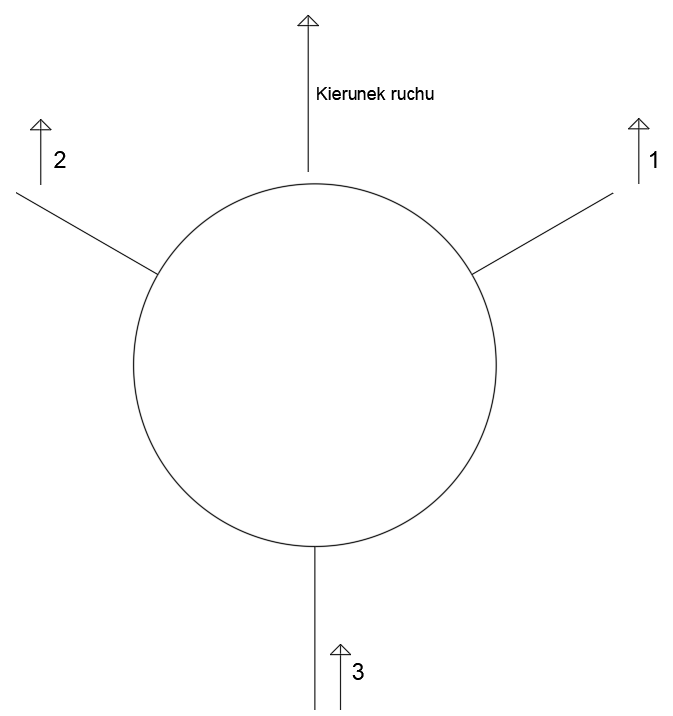
\includegraphics[width=0.4\textwidth]{img/walking_schematic.png}
\centering
\caption{Kolejność przestawiania nóg podczas chodu}
\label{walking_schematic}
\end{figure}

Ta konkretna kolejność przestawiania nóg została wymyślona raczej przypadkowo. Nie wydaje się żeby kolejność w jakiej te nogi są przestawiane miała znaczenie, ważniejsze jest aby każda noga osobno przemieściła się w konkretnym kierunku.\\

% \section{Inne algorytmy}
% Ponieważ zgodnie z najprostrzą kombinatoryką możemy przestawić w jednym momencie albo jedną nogę albo dwie nogi, to mogą istnieć jedynie te dwa algorytmy i ich modyfikacje. Oczywiście w ramach tych modyfikacji może powstać wiele różnych algorytmów, nogę można przestawiać na wiele różnych sposobóe